%%%%%%%%%%%%%%%%%%%%%%%%%%%%%%% beamer %%%%%%%%%%%%%%%%%%%%%%%%%%%%%%%%%%%%%%%%%%%%%%%%%
% To run - pdflatex filename.tex
%      acroread filename.pdf
%%%%%%%%%%%%%%%%%%%%%%%%%%%%%%%%%%%%%%%%%%%%%%%%%%%%%%%%%%%%%%%%%%%%%%%%%%%%%%%%%%%%%%%%

\documentclass[compress,oilve]{beamer}
\mode<presentation>

\usetheme[]{CambridgeUS}
% other themes: AnnArbor, Antibes, Bergen, Berkeley, Berlin, Boadilla, boxes, CambridgeUS, Copenhagen, Darmstadt, default, Dresden, Frankfurt, Goettingen,
% Hannover, Ilmenau, JuanLesPins, Luebeck, Madrid, Maloe, Marburg, Montpellier, PaloAlto, Pittsburg, Rochester, Singapore, Szeged, classic

\usecolortheme{beaver}
% color themes: albatross, beaver, beetle, crane, default, dolphin,  fly, lily, orchid, rose, seagull, seahorse, sidebartab, whale, wolverine

\usefonttheme{professionalfonts}
% font themes: default, professionalfonts, serif, structurebold, structureitalicserif, structuresmallcapsserif


\hypersetup{pdfpagemode=FullScreen} % makes your presentation go automatically to full screen

% define your own colors:
\definecolor{Red}{rgb}{1,0,0}
\definecolor{Blue}{rgb}{0,0,1}
\definecolor{Green}{rgb}{0,1,0}
\definecolor{magenta}{rgb}{1,0,.6}
\definecolor{lightblue}{rgb}{0,.5,1}
\definecolor{lightpurple}{rgb}{0.8, 0.6, 0.9}
\definecolor{gold}{rgb}{.6,.5,0}
\definecolor{orange}{rgb}{1,0.4,0}
\definecolor{hotpink}{rgb}{1,0,0.5}
\definecolor{newcolor2}{rgb}{.5,.3,.5}
\definecolor{newcolor}{rgb}{0,.3,1}
\definecolor{newcolor3}{rgb}{1,0,.35}
\definecolor{darkgreen1}{rgb}{0, .35, 0}
\definecolor{darkgreen}{rgb}{0, .6, 0}
\definecolor{darkred}{rgb}{.75,0,0}
\definecolor{skyblue}{HTML}{75bbfd}

\definecolor{olive}{cmyk}{0.64,0,0.95,0.4}
\definecolor{purpleish}{cmyk}{0.75,0.75,0,0}

% can also choose different themes for the "inside" and "outside"

% \usepackage{beamerinnertheme_______}
% inner themes include circles, default, inmargin, rectangles, rounded

% \usepackage{beamerouterthemesmoothbars}
% outer themes include default, infolines, miniframes, shadow, sidebar, smoothbars, smoothtree, split, tree


\useoutertheme[subsection=true, height=40pt]{smoothbars}

% to have the same footer on all slides
%\setbeamertemplate{footline}[text line]{STUFF HERE!}
\setbeamertemplate{footline}[text line]{} % makes the footer EMPTY
% include packages
%

%show the page numbers in footnote
%\addtobeamertemplate{navigation symbols}{}{%
%	\usebeamerfont{footline}%
%	\usebeamercolor[fg]{footline}%
%	\hspace{1em}%
%	\insertframenumber/\inserttotalframenumber
%}

\setbeamercolor{footline}{fg=purpleish}
\setbeamerfont{footline}{series=\bfseries}

%add color to curent subsection
\setbeamertemplate{section in head/foot}{\hfill\tikz\node[rectangle, fill=darkred, rounded corners=1pt,inner sep=1pt,] {\textcolor{white}{\insertsectionhead}};}
\setbeamertemplate{section in head/foot shaded}{\textcolor{darkred}{\hfill\insertsectionhead}}

% Remove bullet of subsections
\setbeamertemplate{headline}
{%
	\begin{beamercolorbox}{section in head/foot}
		\insertsectionnavigationhorizontal{\textwidth}{}{}
	\end{beamercolorbox}%
}


% modify headlline, specially headline size
\setbeamertemplate{headline}{%
	\leavevmode%
	\hbox{%
		\begin{beamercolorbox}[wd=\paperwidth,ht=3.5ex,dp=1.125ex]{palette quaternary}%
			\insertsectionnavigationhorizontal{\paperwidth}{}{\hskip0pt plus1filll}
		\end{beamercolorbox}%
	}
}

\setbeamertemplate{footline}{%
	\leavevmode%
	\hbox{\begin{beamercolorbox}[wd=.5\paperwidth,ht=2.5ex,dp=1.125ex,leftskip=.3cm plus1fill,rightskip=.3cm]{author in head/foot}%
			\usebeamerfont{author in head/foot}\insertshortauthor ~ \insertshortinstitute
		\end{beamercolorbox}%
		\begin{beamercolorbox}[wd=.5\paperwidth,ht=2.5ex,dp=1.125ex,leftskip=.3cm,rightskip=.3cm plus1fil]{title in head/foot}%
			\usebeamerfont{title in head/foot}\insertshorttitle\hfill\insertframenumber\,/\,\inserttotalframenumber
	\end{beamercolorbox}}%
	\vskip0pt%
}


%\setbeamertemplate{navigation symbols}{}

\title{Generalization Error}
\author{ML Instruction Team, Fall 2022}
\institute[]{CE Department \newline  Sharif University of Technology \newline \newline}
\date[\today]{}
%\titlegraphic{\includegraphics[scale=.35]{example-image}}



%Write \usepackage{etex} just after the \documentclass line (it should be the first loaded package).
\usepackage{etex}
\usepackage{subcaption}
\usepackage{multicol}
\usepackage{amsmath}
\usepackage{epsfig}
\usepackage{graphicx}
\usepackage[all,knot]{xy}
\xyoption{arc}
\usepackage{url}
\usepackage{multimedia}
\usepackage{hyperref}
\hypersetup{colorlinks,linkcolor=blue,citecolor=redorange,urlcolor=darkred}
\usepackage{multirow}
\usepackage[font={scriptsize}]{caption}
\usepackage{pgf}
\usepackage{fontspec}
%\setsansfont[Scale=MatchLowercase, BoldFont = * Bold, ItalicFont = * Italic]{Caladea}

%\usepackage{enumitem,xcolor}
%\newcommand{\labelitemi}{$\blacksquare$}
%\newcommand{\labelitemii}{$\diamond$}
%\newcommand{\labelitemiii}{$\square$}
%\newcommand{\labelitemiv}{$\ast$}
%\setbeamercolor*{item}{fg=red}


\usefonttheme{professionalfonts} 
\setbeamertemplate{itemize item}{\color{skyblue}$\blacksquare$}
\setbeamertemplate{itemize subitem}{\color{hotpink}$\blacktriangleright$}
\setbeamertemplate{itemize subsubitem}{\color{orange}$\bullet$}


\usepackage{anyfontsize}
\usepackage{t1enc}
\usepackage{tikz}
\usetikzlibrary{calc,trees,positioning,arrows,chains,shapes.geometric,decorations.pathreplacing,decorations.pathmorphing,shapes,matrix,shapes.symbols}


\usepackage{xcolor}
\newcommand{\tc}[2]{
	\textcolor{#1}{#2}
}

\newtheorem{proposition}[theorem]{Proposition}
\newtheorem{remark}[theorem]{Remark}
\newtheorem{assumption}[theorem]{Assumption}

%\usepackage{fontspec,unicode-math}
%\setmainfont[Scale=0.9]{Nimbus Roman No9 L}
%\setmonofont[Scale=0.9]{Monaco}
\setsansfont[Scale=1]{Times New Roman}

\newcommand{\vect}[1]{\boldsymbol{#1}}

\definecolor{strings}{rgb}{.624,.251,.259}
\definecolor{keywords}{rgb}{.224,.451,.686}
\definecolor{comment}{rgb}{.322,.451,.322}

%\usepackage{smartdiagram}
%\usesmartdiagramlibrary{additions}


%%%%%%%%%%%%%%%%%%%%%%%%%%%%%%%%%%%%%%%%%%%%%%%%%%%%%%%%%%%%%%%%%%%%%%%%%%%%%%%%%%%%%%%%%%%%
%%%%%%%%%%%%%%%%%%%%%%%%%%%%%% Title Page Info %%%%%%%%%%%%%%%%%%%%%%%%%%%%%%%%%%%%%%%%%%%
%%%%%%%%%%%%%%%%%%%%%%%%%%%%%%%%%%%%%%%%%%%%%%%%%%%%%%%%%%%%%%%%%%%%%%%%%%%%%%%%%%%%%%%%%%


%%%%%%%%%%%%%%%%%%%%%%%%%%%%%%%%%%%%%%%%%%%%%%%%%%%%%%%%%%%%%%%%%%%%%%%%%%%%%%%%%%%%%%%%%%
%%%%%%%%%%%%%%%%%%%%%%%%%%%%%% Begin Your Document %%%%%%%%%%%%%%%%%%%%%%%%%%%%%%%%%%%%%%%
%%%%%%%%%%%%%%%%%%%%%%%%%%%%%%%%%%%%%%%%%%%%%%%%%%%%%%%%%%%%%%%%%%%%%%%%%%%%%%%%%%%%%%%%%%
\begin{document}
	
%%%%%%%%%%%%%%%%%%%%%%%%%%%%%%%%%%%%%%%%%%%%%%%%%%%%%%%%%%%%%%%%%%%%%%%%%%%%%%%%%%%%%%%%%%
	\fontsize{9}{9}
\begin{frame}[noframenumbering, plain]
	\titlepage
\end{frame}

%%%%%%%%%%%%%%%%%%%%%%%%%%%%%%%%%%%%%%%%%%%%%%%%%%%%%%%%%%%%%%%%%%%%%%%%%%%%%%%%%%%%%%%%%%
\section{Generalization Error}
%%%%%%%%%%%%%%%%%%11111111111111111%%%%%%%%%%%%%%%%%%%%%%%%%%%%%%%%%%%%%%%%%%%%%%%%%%%%%%%%%%%%%%
\frame{\frametitle{Generalization Performance}
\begin{figure}
				\href{https://medium.com/@prasoonthakur5/machinelearning-ab9c3c13293d}{
				\centering
				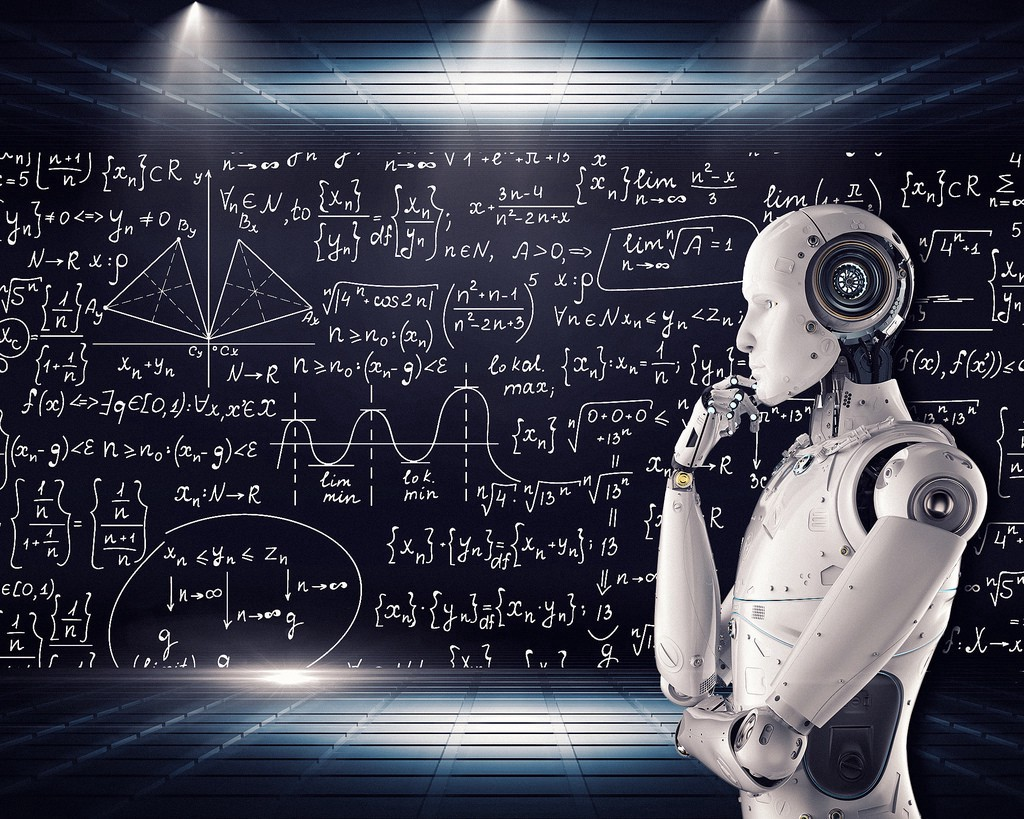
\includegraphics[width=9cm, height=5.625cm]{images/learning.jpeg}}
			\end{figure}
\centering
\vspace\textbf{When can we say the machine has learned?}
}

%%%%%%%%%%%%%%%2222222222222222222222%%%%%%%%%%%%%%%%%%%%%%%%%%%%%%%%%%%%%%%%%%%%%%%%%%%%%%%%%%%%%%%%%
\frame{\frametitle{Assumptions}

\begin{itemize}
\item Inputs are independent, and training and test examples are identically distributed (i.i.d).
\smallskip

\item For some random model that has not been fitted to the training set, we expect both the training and test error to be equal. \smallskip
\item The training error or accuracy provides an (optimistically) biased estimate of the generalization performance.
\end{itemize}
}
%%%%%%%%%%%%%%33333333333333333333%%%%%%%%%%%%%%%%%%%%%%%%%%%%%%%%%%%%%%%%%%%%%%%%%%%%%%%%%%######
\frame{\frametitle{Terminology }

Point estimator θ of some parameter θ

\begin{equation}
\mathrm{\textbf{Bias} } = E [\hat{f}]  - f
\end{equation}
\begin{equation}
\mathrm{\textbf{Var} }  = E \left[\hat{f} ^2\right]  -  \left(E [\hat{f}] \right)^2
\end{equation}
\begin{equation}
\text{Noise: } \sigma^2 = E\left[\epsilon^2\right]
\end{equation}
\begin{equation}
\text{target function:} \:\:  y = \mathrm {f}(x) + \epsilon
\end{equation}
\begin{equation}
\text{predicted target value:} \:\: \hat{y} = \hat{f}(x) 
\end{equation}
\begin{equation}
\text{mean squared loss:} \:\:   MSE  =  E\left[\left(y - \hat{y}\right)^2\right]
\end{equation}}

%%%%%%%%%%%%%%%4444444444444444444%%%%%%%%%%%%%%%%%%%%%%%%%%%%%%%%%%%%%%%%%%%%%%%%%%%%%%%%%######
\frame{\frametitle{ Bias-Variance Decomposition of Squared Error }
\begin{align} MSE =
E\big[(y - \hat{y})^2\big]
 & = E\big[(f+\epsilon  - \hat{f} )^2\big] \\[5pt]
 & = E\big[(f+\epsilon  - \hat{f} +E[\hat{f}]-E[\hat{f}])^2\big] \\[5pt]
 & = (f-E[\hat{f}])^2+E[\epsilon^2]+E\big[(E[\hat{f}]- \hat{f})^2\big]\\[5pt]
 & = \mathrm{\textbf{Bias} }+\mathrm{\textbf{Var} }+\sigma^2 
\end{align}
}
%%%%%%%%%%%%%%%%%%55555555555555555555%%%%%%%%%%%%%%%%%%%%%%%%%%%%%%%%%%%%%%%%%%%%%%%%%%%%%%######
\frame{\frametitle{ Bias-Variance Decomposition }


% \centering
 {\fontsize{.7cm}{0.7cm}\selectfont $$ \textbf{ Loss = \tc{Blue}{Bias} + \tc{Red}{Variance} + Noise }$$\par}
\bigskip

\begin{itemize}
\item Decomposition of the loss into bias and variance help us understand learning algorithms, concepts are correlated to underfitting and overfitting
\item Helps explain why ensemble methods (last lecture) might perform better than single models
\end{itemize}

}

%%%%%%%%%%%%%%%%%6666666666666666666%%%%%%%%%%%%%%%%%%%%%%%%%%%%%%%%%%%%%%%%%%%%%%%%%%%%%%%%%%%%%%%
\frame{\frametitle{Underfitting VS Overfitting  }

\begin{itemize}
\item \tc{newcolor}{Underfitting}: both training and test error are large\smallskip
\item \tc{newcolor3}{Overfitting}: gap between training and test error 
\end{itemize}
% \item 
% \item 
\begin{figure}
		\href{https://srdas.github.io/DLBook/ImprovingModelGeneralization.html}{
				\centering
				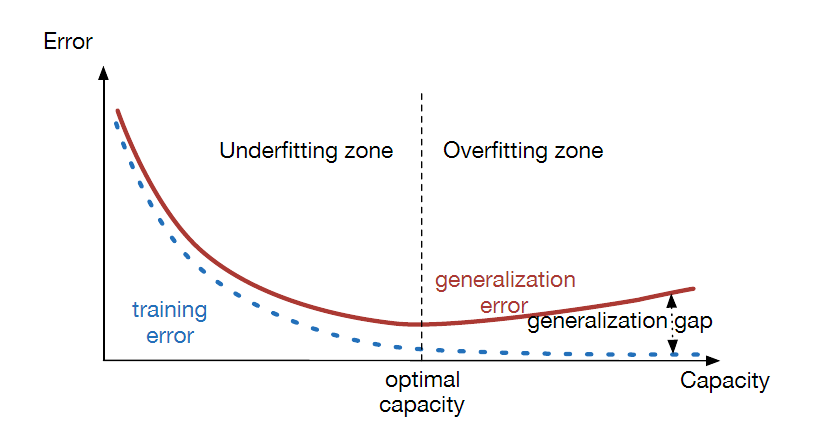
\includegraphics[width=12cm]{Figs/Generalization Error.png}}
			\end{figure}
}           
%%%%%%%%%%%%%%%%%%777777777777777777%%%%%%%%%%%%%%%%%%%%%%%%%%%%%%%%%%%%%%%%%%%%%%%%%%%%%%######
\frame{\frametitle{ Bias-Variance Trade-off }

\begin{figure}
		\href{https://www.geeksforgeeks.org/ml-bias-variance-trade-off/}{
				\centering
				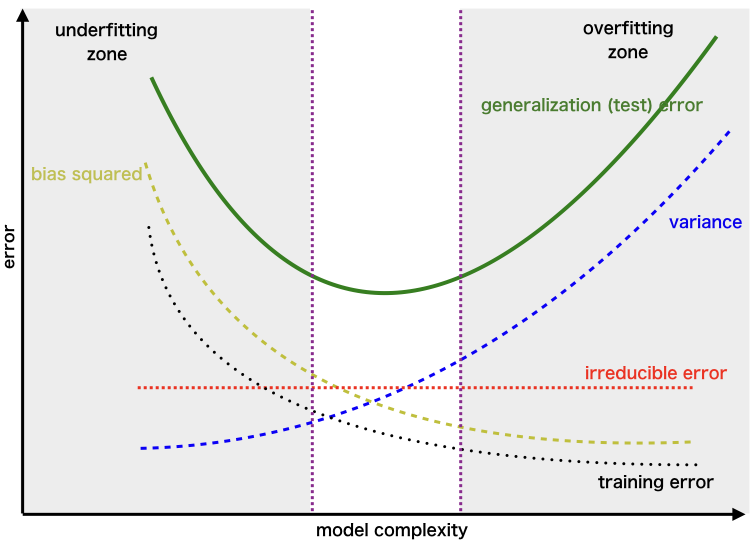
\includegraphics[width=10cm]{Figs/ERROR.png}}
			\end{figure}
	
}

%%%%%%%%%%%%%%%%%%%888888888888888%%%%%%%%%%%%%%%%%%%%%%%%%%%%%%%%%%%%%%%%%%%%%%%%%%%%%%%%%%%%%
\section{Bias-Variance Trade-off}


%%%%%%%%%%%%%%%99999999999999%%%%%%%%%%%%%%%%%%%%%%%%%%%%%%%%%%%%%%%%%%%%%%%%%%%%%%%%%######
\frame{\frametitle{ Bias-Variance Trade-off }
\begin{figure}
		\href{https://github.com/rasbt/stat479-machine-learning-fs18/blob/master/08_eval-intro/08_eval-intro_notes.pdf}{
				\centering
				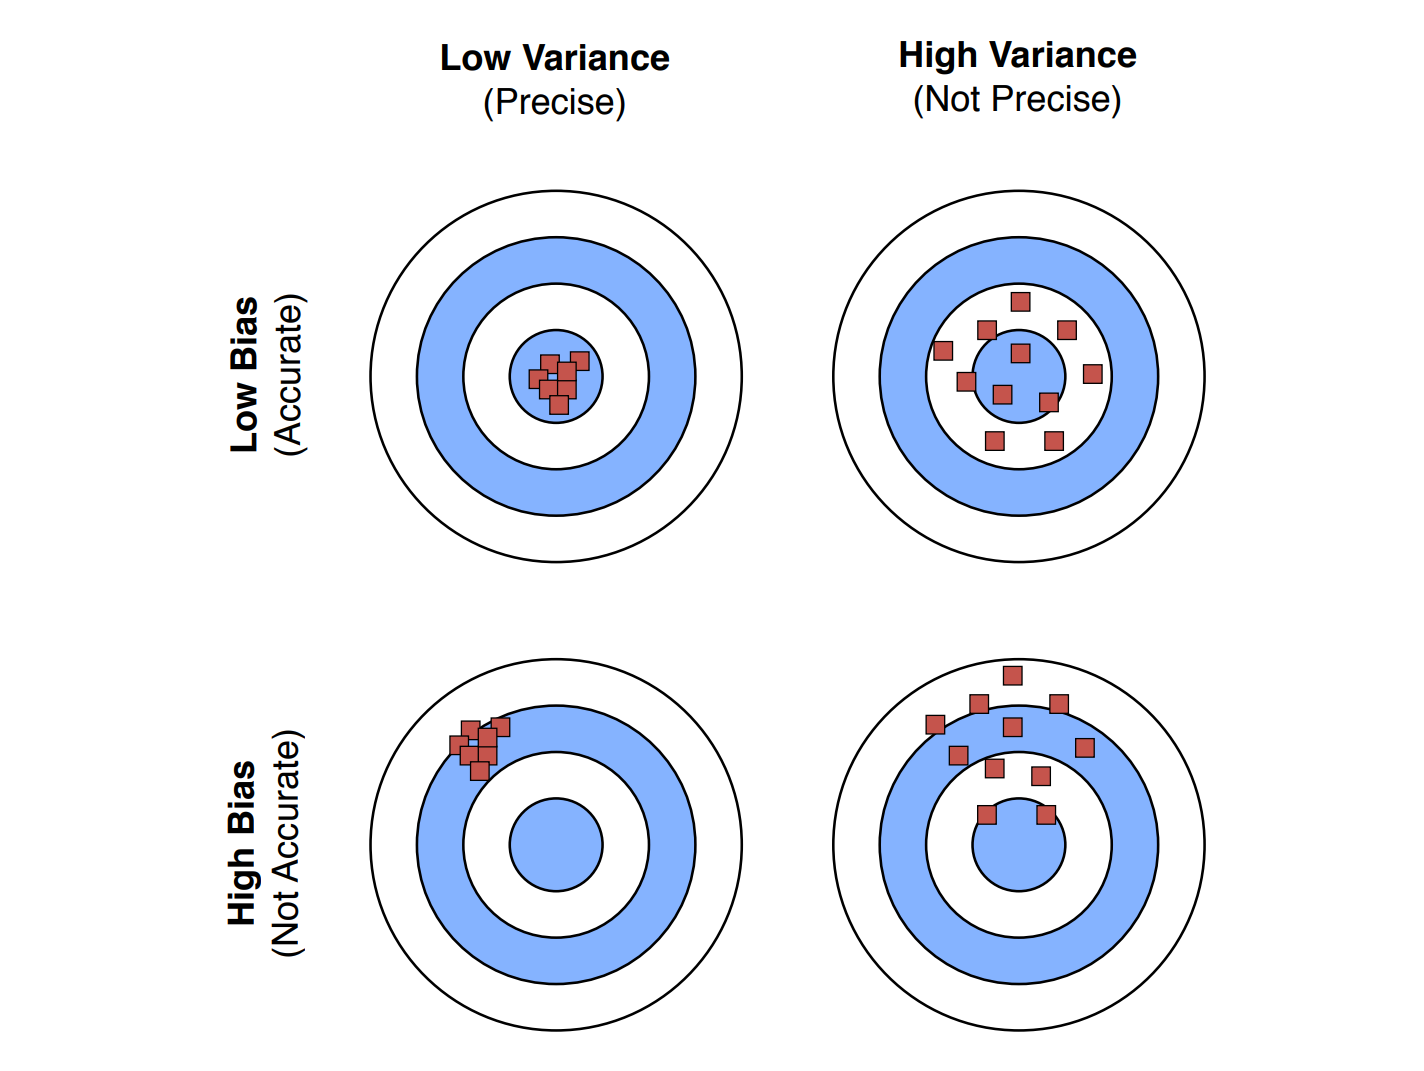
\includegraphics[width=9cm]{Figs/Bias-Variance Intuition.png}}
			\end{figure}
	
}
%%%%%%%%%%%%%%%%%%%%%%%%%%%%%%%%%%%%%%%%%%%%%%%%%%%%%%%%%%%%%%%%%%%%%%%%######
% \frame{\frametitle{ Bias-Variance Trade-off }

% % \centering
% % \large  {Bias-Variance Intuition}

% \begin{pspicture}(2.45,3.45)
%   \target(0.25,0)
%   \target(2.05,0)
%   \target(0.25,1.8)
%   \target(2.05,1.8)
%   \dots[0.12](0.95,1.1)
%   \dots[0.1](0.92,2.53)
%   \dots[0.3](2.5,1.15)
%   \dots[0.3](2.7,2.5)
%   \rput{90}(0.05,0.7){High Bias}
%   \rput{90}(0.05,2.5){Low Bias}
%   \rput(0.95,3.4){Low Variance}
%   \rput(2.75,3.4){High Variance}
% \end{pspicture}

% }

%%%%%%%%%%%%%%%%%%%%%%%%%%%%%%%%%%%%%%%%%%%%%%%%%%%%%%%%%%%%%%%%%%%%%%%%######
\frame{\frametitle{ Bias-Variance Trade-off }

\begin{figure}
		\href{https://github.com/rasbt/stat479-machine-learning-fs18/blob/master/08_eval-intro/08_eval-intro_notes.pdf}{
				\centering
				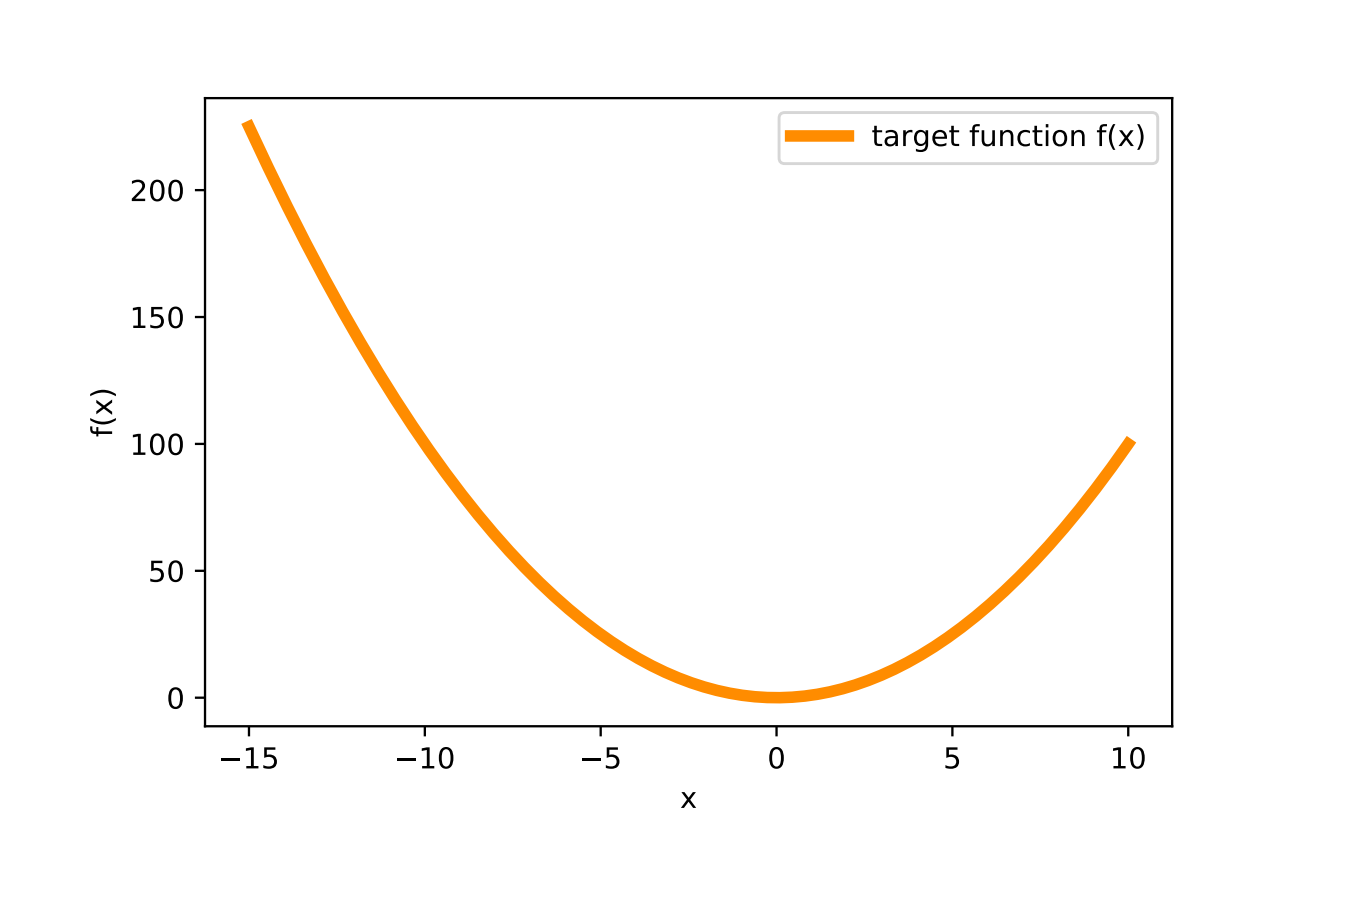
\includegraphics[width=10cm]{Figs/1.png}}
			\end{figure}

	
}
%%%%%%%%%%%%%%%%%%%%%%%%%%%%%%%%%%%%%%%%%%%%%%%%%%%%%%%%%%%%%%%%%%%%%%%%######
\frame{\frametitle{ Bias-Variance Trade-off }

\begin{figure}
		\href{https://github.com/rasbt/stat479-machine-learning-fs18/blob/master/08_eval-intro/08_eval-intro_notes.pdf}{
				\centering
				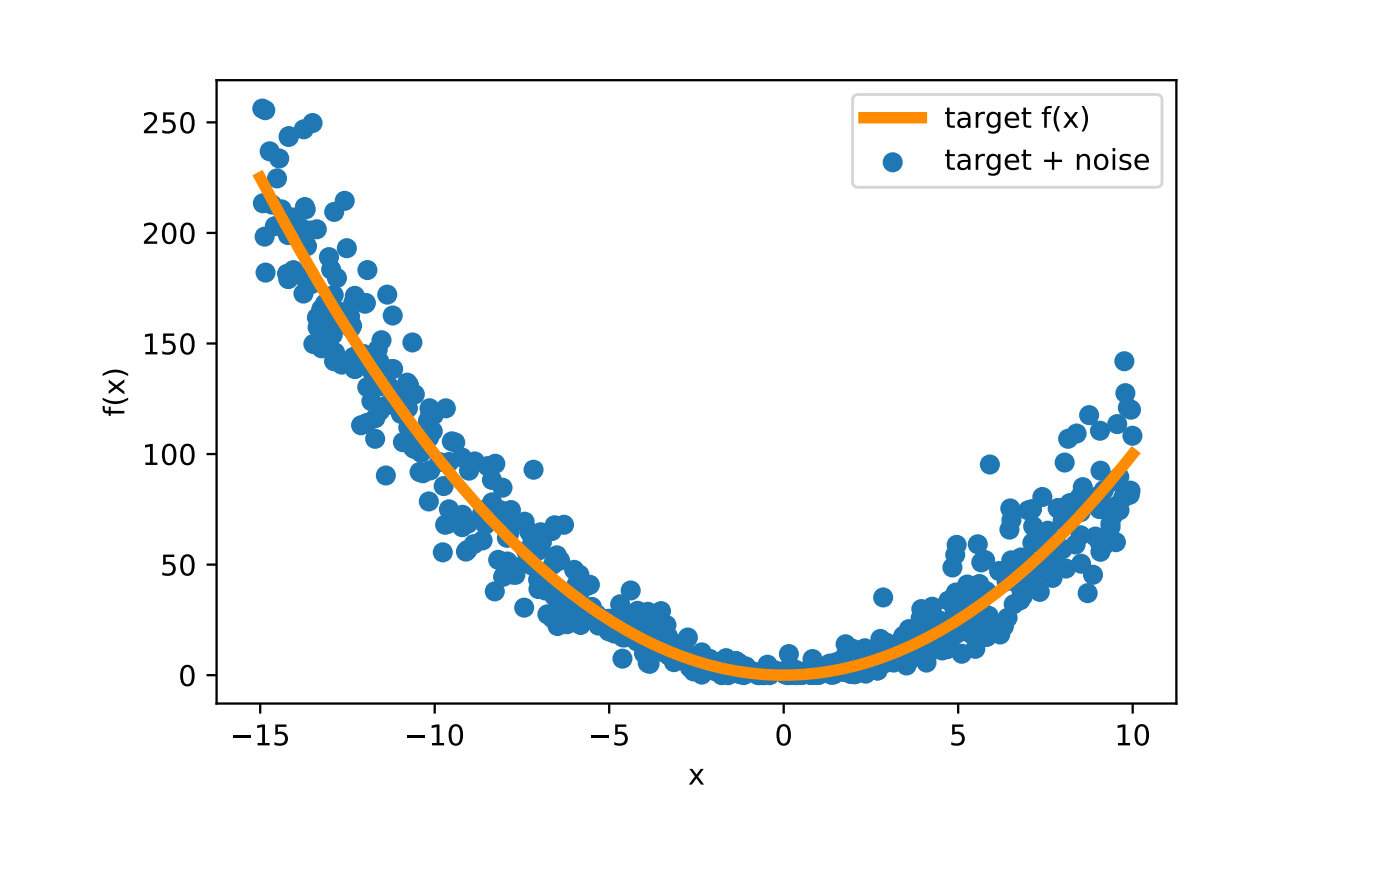
\includegraphics[width=10cm]{Figs/2.png}}
			\end{figure}

	
}
%%%%%%%%%%%%%%%%%%%%%%%%%%%%%%%%%%%%%%%%%%%%%%%%%%%%%%%%%%%%%%%%%%%%%%%%######
\frame{\frametitle{ Bias-Variance Trade-off }

\begin{figure}
		\href{https://github.com/rasbt/stat479-machine-learning-fs18/blob/master/08_eval-intro/08_eval-intro_notes.pdf}{
				\centering
				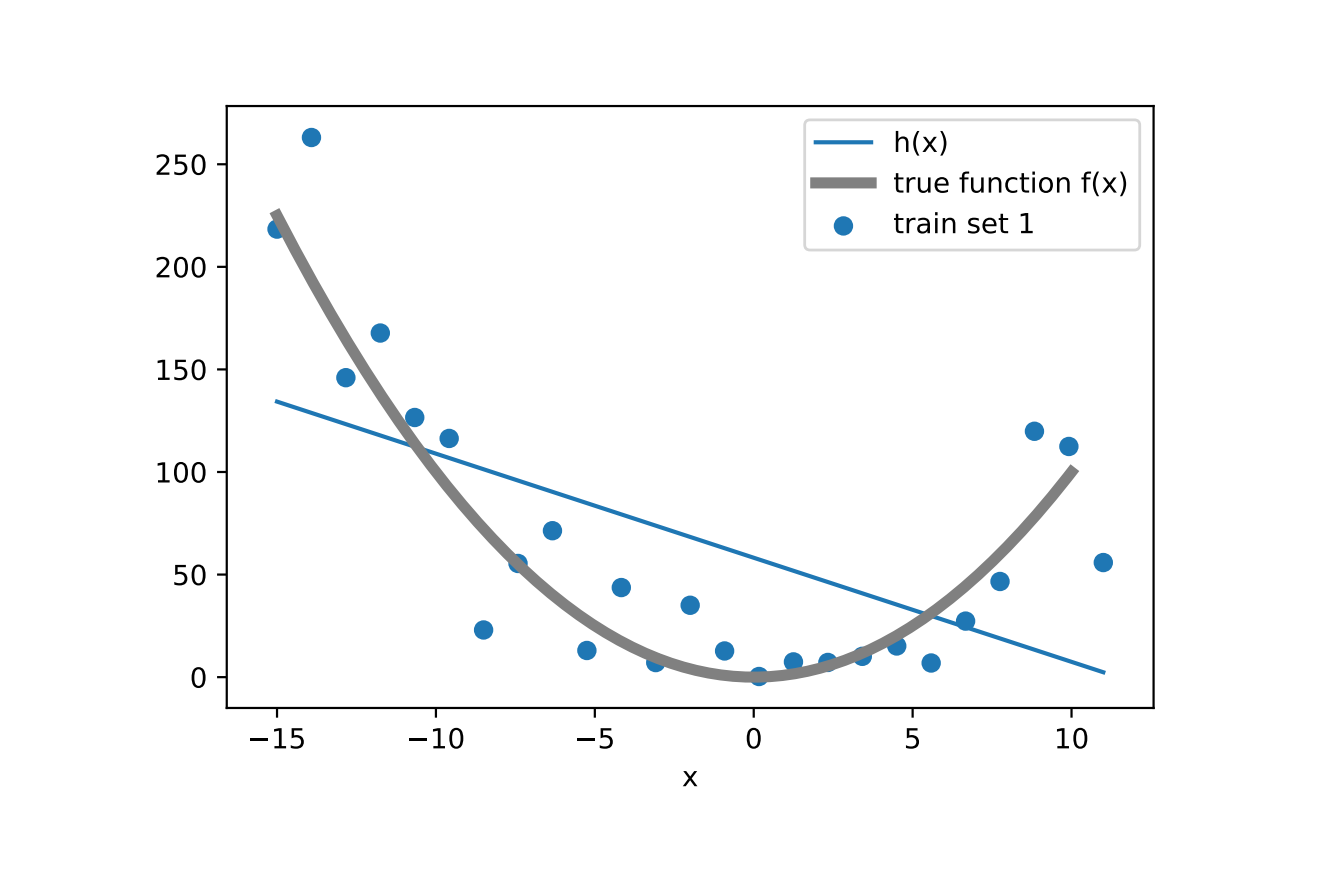
\includegraphics[width=10cm]{Figs/3.png}}
			\end{figure}

	
}
%%%%%%%%%%%%%%%%%%%%%%%%%%%%%%%%%%%%%%%%%%%%%%%%%%%%%%%%%%%%%%%%%%%%%%%%######
\frame{\frametitle{ Bias-Variance Trade-off }

\begin{figure}
		\href{https://github.com/rasbt/stat479-machine-learning-fs18/blob/master/08_eval-intro/08_eval-intro_notes.pdf}{
				\centering
				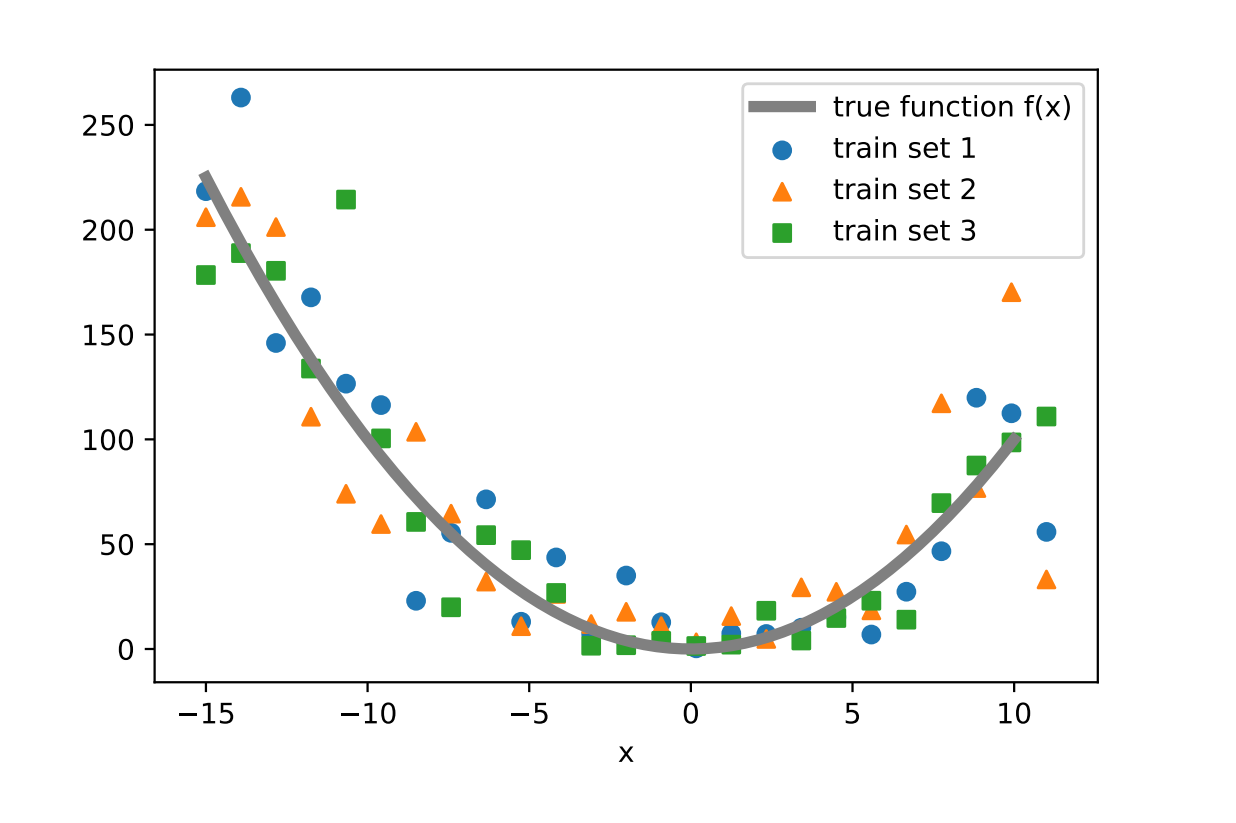
\includegraphics[width=10cm]{Figs/4.png}}
			\end{figure}

	
}
%%%%%%%%%%%%%%%%%%%%%%%%%%%%%%%%%%%%%%%%%%%%%%%%%%%%%%%%%%%%%%%%%%%%%%%%######
\frame{\frametitle{ Bias-Variance Trade-off }

\begin{figure}
		\href{https://github.com/rasbt/stat479-machine-learning-fs18/blob/master/08_eval-intro/08_eval-intro_notes.pdf}{
				\centering
				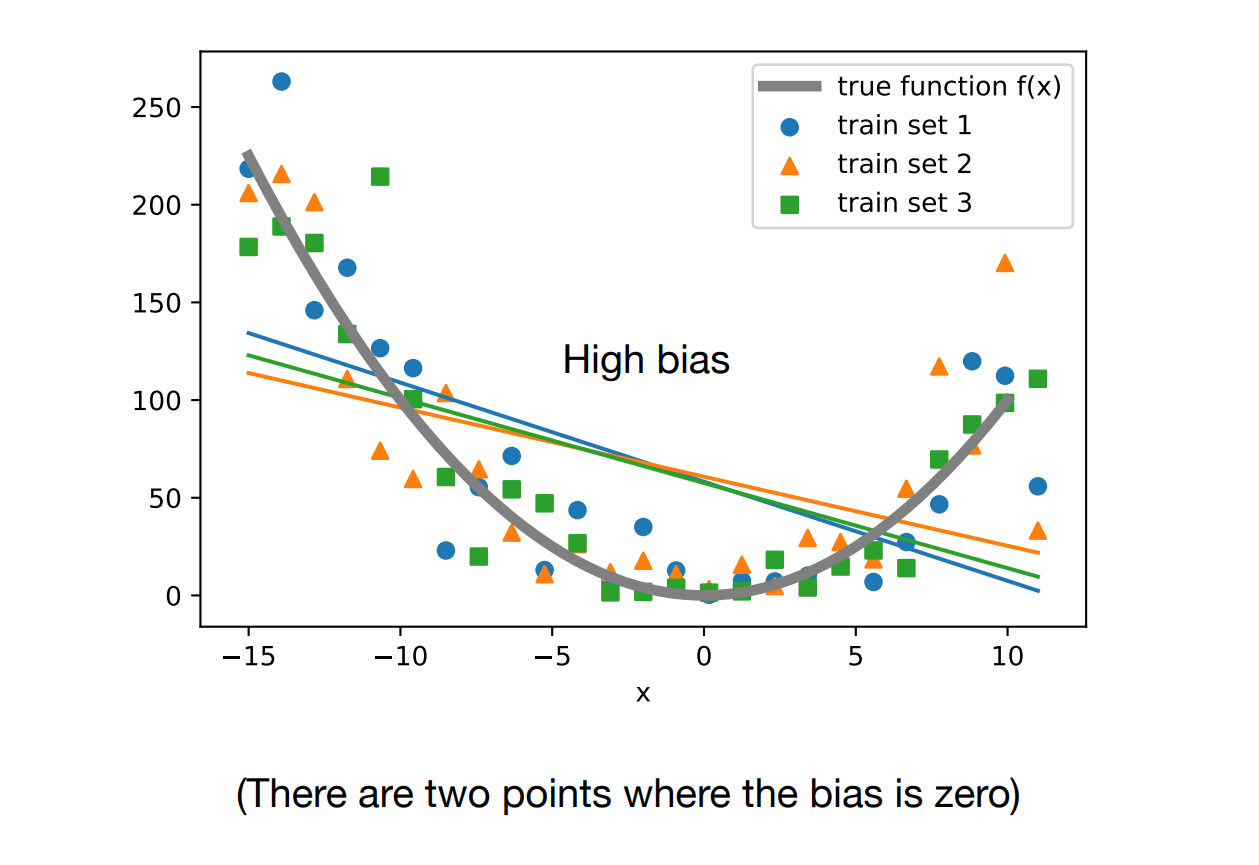
\includegraphics[width=10cm]{Figs/5.png}}
			\end{figure}

	
}
%%%%%%%%%%%%%%%%%%%%%%%%%%%%%%%%%%%%%%%%%%%%%%%%%%%%%%%%%%%%%%%%%%%%%%%%######
\frame{\frametitle{ Bias-Variance Trade-off }

\begin{figure}
		\href{https://github.com/rasbt/stat479-machine-learning-fs18/blob/master/08_eval-intro/08_eval-intro_notes.pdf}{
				\centering
				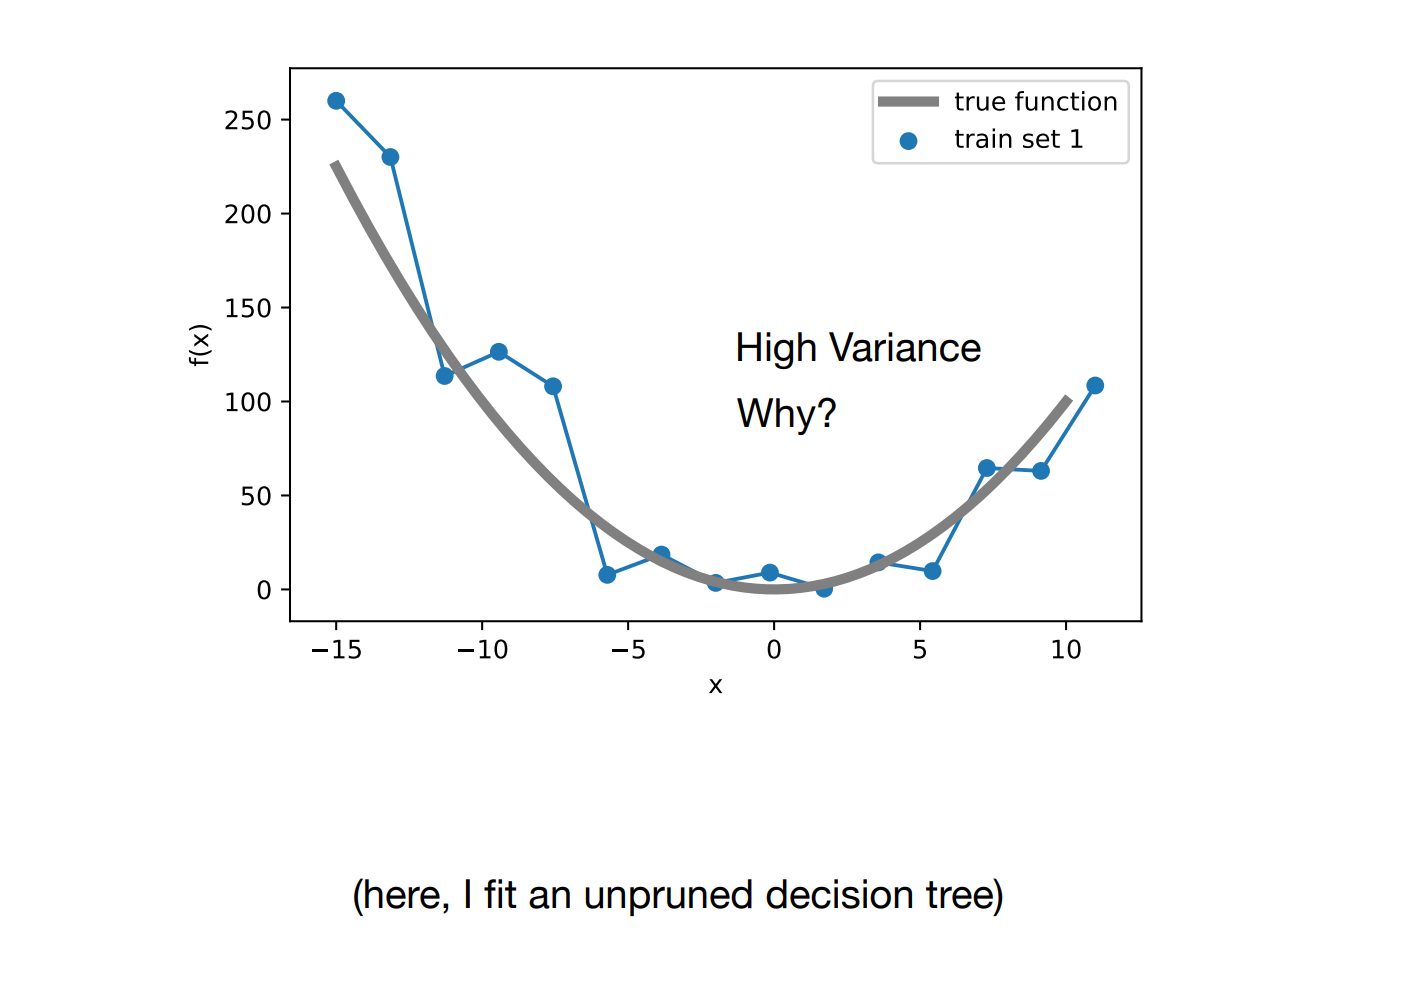
\includegraphics[width=10cm]{Figs/6.png}}
			\end{figure}

	
}
%%%%%%%%%%%%%%%%%%%%%%%%%%%%%%%%%%%%%%%%%%%%%%%%%%%%%%%%%%%%%%%%%%%%%%%%######
\frame{\frametitle{ Bias-Variance Trade-off }

\begin{figure}
		\href{https://github.com/rasbt/stat479-machine-learning-fs18/blob/master/08_eval-intro/08_eval-intro_notes.pdf}{
				\centering
				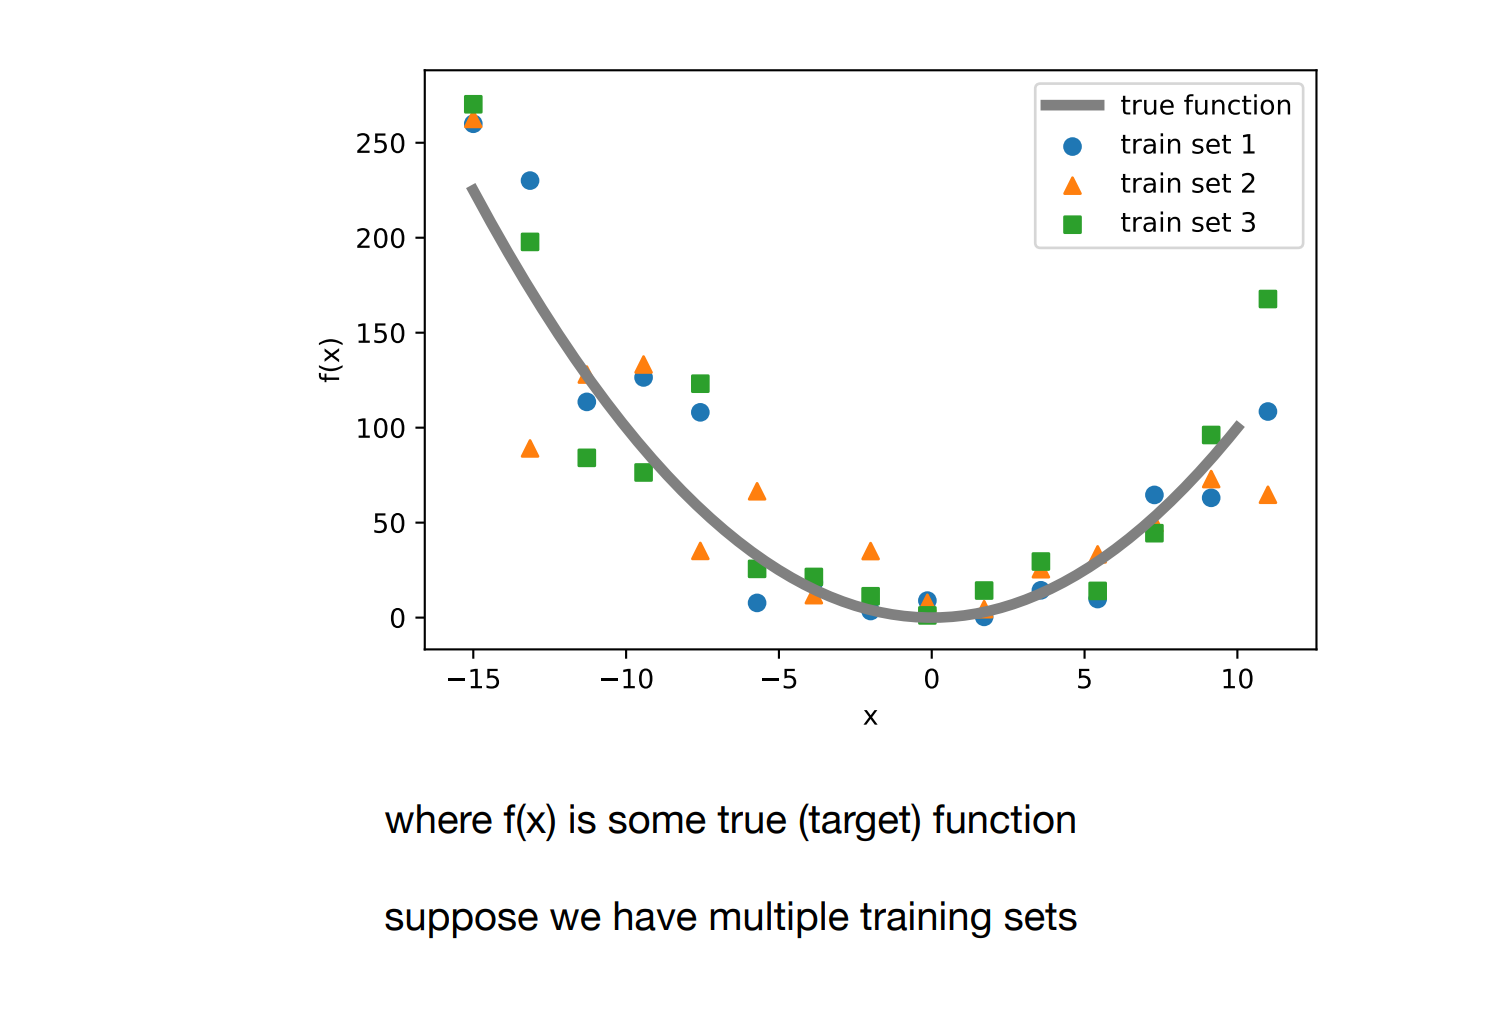
\includegraphics[width=10cm]{Figs/7.png}}
			\end{figure}

	
}
%%%%%%%%%%%%%%%%%%%%%%%%%%%%%%%%%%%%%%%%%%%%%%%%%%%%%%%%%%%%%%%%%%%%%%%%######
\frame{\frametitle{ Bias-Variance Trade-off }

\begin{figure}
		\href{https://github.com/rasbt/stat479-machine-learning-fs18/blob/master/08_eval-intro/08_eval-intro_notes.pdf}{
				\centering
				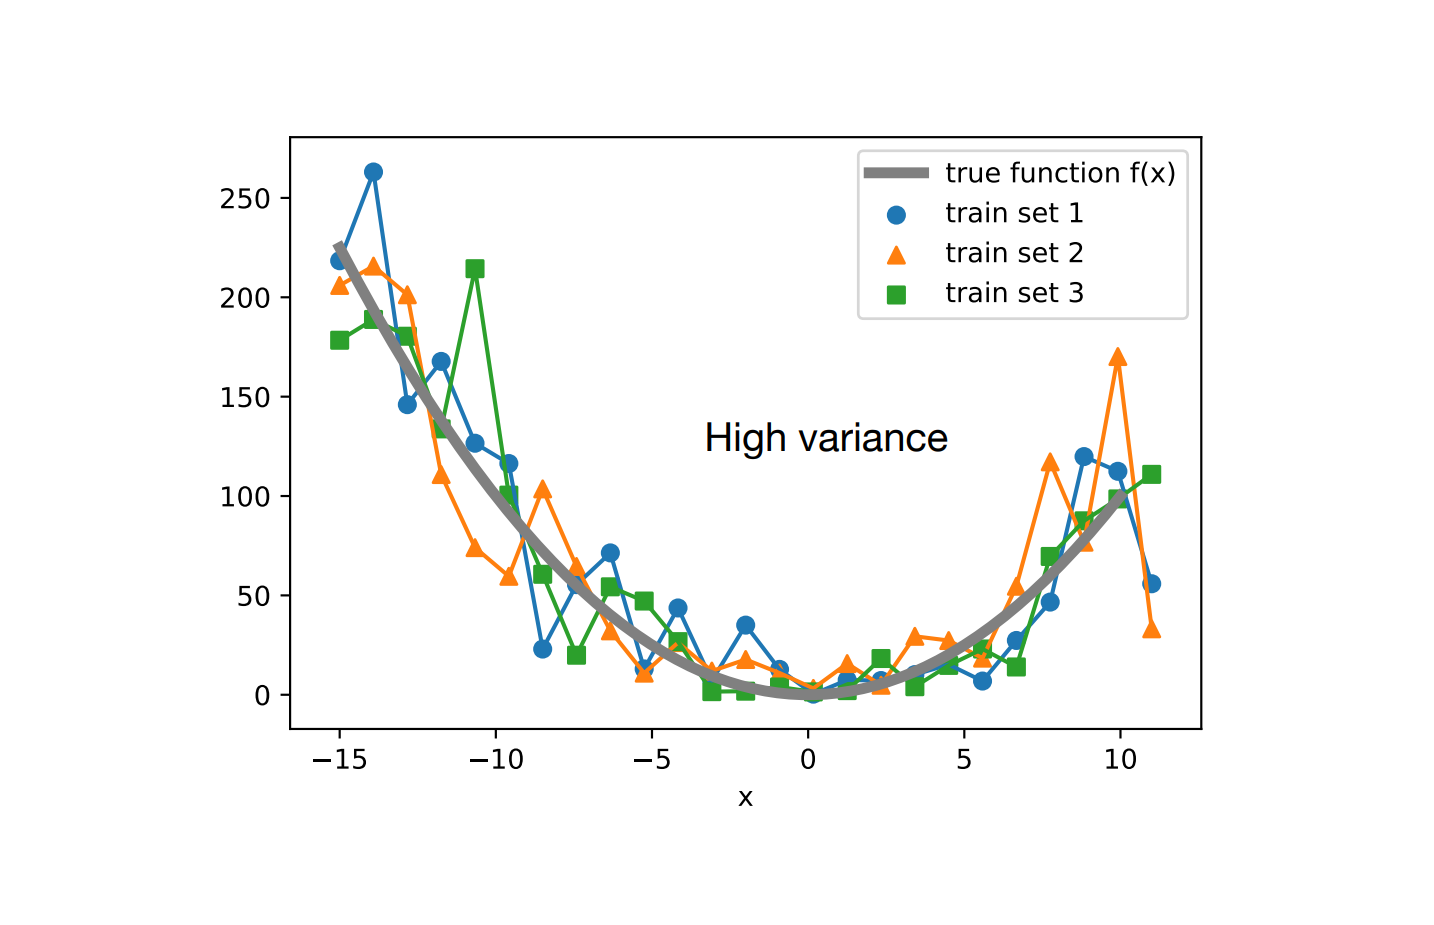
\includegraphics[width=10cm]{Figs/8.png}}
			\end{figure}

	
}
%%%%%%%%%%%%%%%%%%%%%%%%%%%%%%%%%%%%%%%%%%%%%%%%%%%%%%%%%%%%%%%%%%%%%%%%######
\frame{\frametitle{ Bias-Variance Trade-off }

\begin{figure}
		\href{https://github.com/rasbt/stat479-machine-learning-fs18/blob/master/08_eval-intro/08_eval-intro_notes.pdf}{
				\centering
				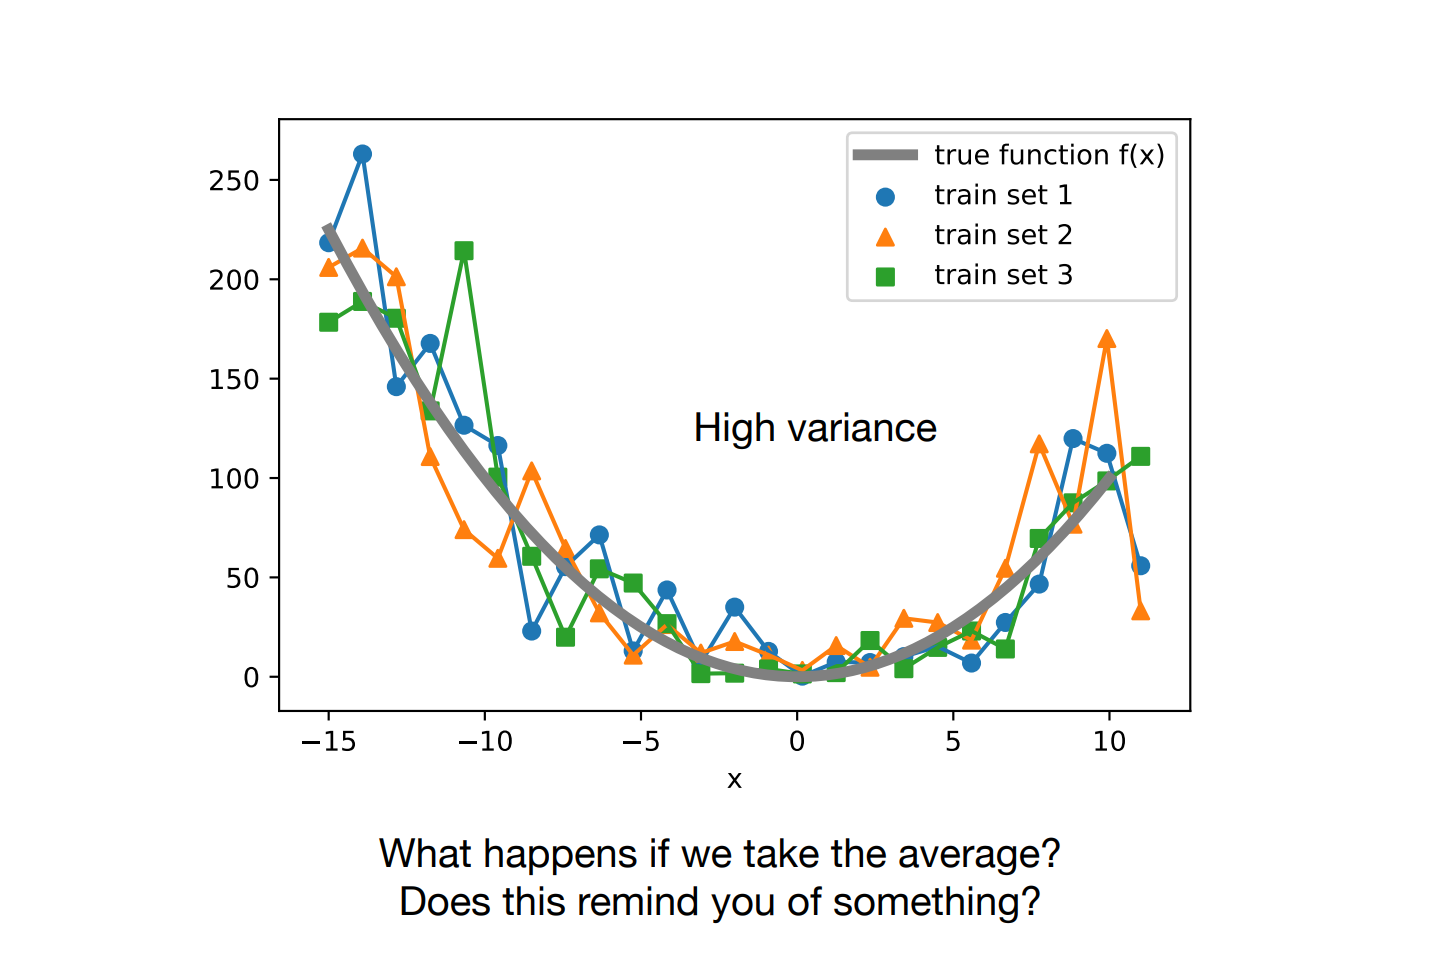
\includegraphics[width=10cm]{Figs/9.png}}
			\end{figure}

	
}

%%%%%%%%%%%%%%%%%%%%%%%%%%%%%%%%%%%%%%%%%%%%%%%%%%%%%%%%%%%%%%%%%%%%%%%%%%%%%%%

% \frame{\frametitle{Train, Validation and Test Errors}
	
	
% \begin{itemize}
% 	\item One
% 	\begin{itemize}
% 		\item One
% 		\item Two
% 		\item Three
% 	\end{itemize}

% 	\item 
% 	For two-dimensional tensors, we have a corresponding sum with indices $(a, b)$ for $f$ and $(i-a, j-b)$ for $g$, respectively:
% 	$$
% 	(f * g)(i, j)=\sum_a \sum_b f(a, b) g(i-a, j-b)
% 	$$
	
% 	\item 
	
% 	It is given by,
% 	$$
% 	\left.w_{t+1}=w_t-\left(\alpha_t / \sqrt{\left(v_t\right.}\right)+e\right) *\left(\delta L / \delta w_t\right)
% 	$$
% 	where,
% 	$$
% 	v_t=\beta * v_t+(1-\beta) *\left(\delta L / \delta w_t\right)^2
% 	$$
% \end{itemize}	
	
}

%%%%%%%%%%%%%%%%%%%%%%%%%%%%%%%%%%%%%%%%%%%%%%%%%%%%%%%%%%%%%%%%%%%%%%%%%%%%%%%%%%%%%%%%%%%%%%%


\frametitle{Final Notes}
\centering
\vspace{50 pt}
\textbf{Thank You!}

\vspace{50pt}
\textbf{Any Question?}
%%%%%%%%%%%%%%%%%%%%%%%%%%%%%%%%%%%%%%%%%%

\end{document}
